% Figure 1 (fig:schematic): sketch of the problem. Standalone TikZ; compile with
%   pdflatex -jobname fig1_schematic fig01_schematic.tex      (or: python make_all.py fig01)
\documentclass[border=2pt]{standalone}
\usepackage{amsmath,amssymb,bm}
\usepackage{tikz}
\usepackage{pgfplots}
\pgfplotsset{compat=1.17}
\usetikzlibrary{arrows.meta,patterns,positioning,calc,decorations.pathreplacing,shapes.geometric}
\providecommand{\mathsfbi}[1]{\boldsymbol{\mathsf{#1}}}
\definecolor{cunc}{HTML}{52514E}
\definecolor{clqr}{HTML}{2A78D6}
\definecolor{copt}{HTML}{EB6834}
\definecolor{cvp}{HTML}{D6604D}
\definecolor{cvm}{HTML}{4393C3}
\definecolor{cbox}{HTML}{F2F1EE}
\begin{document}
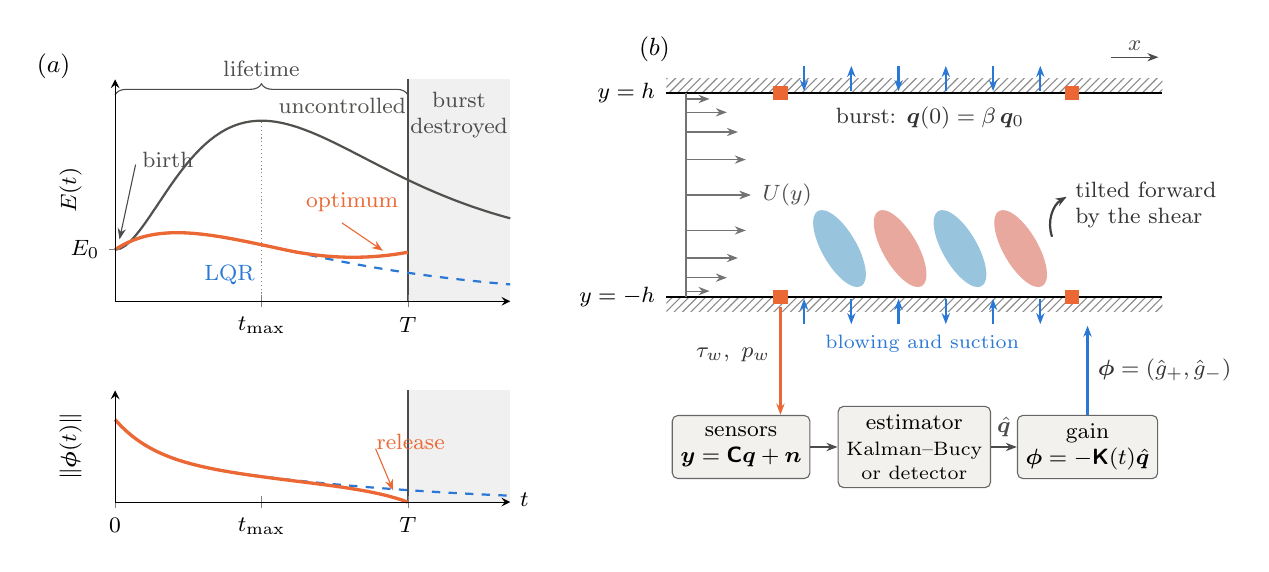
\begin{tikzpicture}[font=\footnotesize, >={Stealth[length=4pt]}]

% =====================================================================================
% (a) life of a burst: energy and control
% =====================================================================================
\begin{axis}[name=energy, at={(0,2.55cm)}, width=6.6cm, height=4.4cm,
    xmin=0, xmax=2.7, ymin=0, ymax=4.3, axis lines=left, xtick={1,2}, xticklabels={$t_{\mathrm{max}}$,$T$},
    ytick={1}, yticklabels={$E_0$}, ylabel={$E(t)$}, ylabel style={at={(-0.06,0.5)}},
    tick label style={font=\footnotesize}, clip=false, axis on top]
  \fill[black!6] (axis cs:2,0) rectangle (axis cs:2.7,4.3);
  \draw[black!45, densely dotted] (axis cs:1,0) -- (axis cs:1,3.5);
  \draw[black!70, thick] (axis cs:2,0) -- (axis cs:2,4.3);
  \addplot[cunc, thick, domain=0:2.7, samples=80] {1+2.5*x^2*exp(2*(1-x))};
  \addplot[clqr, thick, dashed, domain=0:2.7, samples=80] {(1+0.9*x*exp(1-x))*exp(-0.55*x)};
  \addplot[copt, very thick, domain=0:2, samples=80] {(1+0.9*x*exp(1-x))*exp(-0.55*x) + 0.55*(x>1.15)*(x-1.15)^2};
  \node[cunc, anchor=south west] at (axis cs:1.05,3.45) {uncontrolled};
  \node[clqr, anchor=north east] at (axis cs:1.02,0.88) {LQR};
  \node[copt, anchor=south] at (axis cs:1.62,1.55) {optimum};
  \draw[->, copt] (axis cs:1.55,1.52) -- (axis cs:1.83,0.98);
  \node[align=center, anchor=north, black!70] at (axis cs:2.35,4.25) {burst\\destroyed};
  \node[align=center, anchor=west, black!70] at (axis cs:0.12,2.75) {birth};
  \draw[->, black!70] (axis cs:0.14,2.65) -- (axis cs:0.03,1.2);
  \draw[decorate, decoration={brace, amplitude=4pt}, black!70] (axis cs:0,4.0) -- node[above=3pt] {lifetime} (axis cs:2,4.0);
  \node[font=\small] at (axis cs:-0.42,4.55) {($a$)};
\end{axis}
\begin{axis}[name=control, at={(0,0)}, width=6.6cm, height=3.0cm,
    xmin=0, xmax=2.7, ymin=0, ymax=1.15, axis lines=left, xtick={0,1,2}, xticklabels={$0$,$t_{\mathrm{max}}$,$T$},
    ytick=\empty, ylabel={$\|\bm{\phi}(t)\|$}, ylabel style={at={(-0.06,0.5)}}, xlabel={$t$},
    xlabel style={at={(1.0,0.02)}, anchor=west}, tick label style={font=\footnotesize}, clip=false, axis on top]
  \fill[black!6] (axis cs:2,0) rectangle (axis cs:2.7,1.15);
  \draw[black!70, thick] (axis cs:2,0) -- (axis cs:2,1.15);
  \addplot[clqr, thick, dashed, domain=0:2.7, samples=80] {0.85*exp(-3*x)+0.3*x*exp(1-x)*exp(-0.3*x)};
  \addplot[copt, very thick, domain=0:2, samples=120] {(0.85*exp(-3*x)+0.3*x*exp(1-x)*exp(-0.3*x))*(1-exp(-(2-x)/0.22))};
  \node[copt, anchor=west, align=left] at (axis cs:1.72,0.62) {release};
  \draw[->, copt] (axis cs:1.78,0.55) -- (axis cs:1.9,0.12);
\end{axis}

% =====================================================================================
% (b) channel, sensors, actuators and controller
% =====================================================================================
\begin{scope}[shift={(7.0cm,0.25cm)}]
  \def\W{6.3}  % channel length
  \def\H{2.6}  % channel height
  \def\yb{2.35} % bottom wall
  \node[font=\small] at (-0.15,\yb+\H+0.55) {($b$)};
  % walls
  \fill[pattern=north east lines, pattern color=black!45] (0,\yb-0.18) rectangle (\W,\yb);
  \fill[pattern=north east lines, pattern color=black!45] (0,\yb+\H) rectangle (\W,\yb+\H+0.18);
  \draw[thick] (0,\yb) -- (\W,\yb); \draw[thick] (0,\yb+\H) -- (\W,\yb+\H);
  \node[anchor=east] at (-0.02,\yb) {$y=-h$}; \node[anchor=east] at (-0.02,\yb+\H) {$y=h$};
  % mean profile
  \foreach \y/\u in {0.08/0.30, 0.25/0.52, 0.5/0.66, 0.85/0.76, 1.3/0.82} {
      \draw[->, black!55] (0.25,\yb+\y) -- (0.25+\u,\yb+\y);
      \draw[->, black!55] (0.25,\yb+\H-\y) -- (0.25+\u,\yb+\H-\y); }
  \draw[black!55] (0.25,\yb) -- (0.25,\yb+\H);
  \node[black!70, anchor=west] at (1.1,\yb+\H/2) {$U(y)$};
  \draw[->, black!70] (\W-0.65,\yb+\H+0.45) -- node[above=-1pt] {$x$} (\W-0.05,\yb+\H+0.45);
  % burst: backwards-tilted wall-normal velocity (Orr) with streaks, near the lower wall
  \begin{scope}[shift={(3.35,\yb+0.62)}]
    \foreach \dx/\c in {-1.15/cvm, -0.38/cvp, 0.38/cvm, 1.15/cvp} {
      \fill[\c, opacity=0.55, rotate around={30:(\dx,0)}] (\dx,0) ellipse (0.22 and 0.55); }
    \draw[->, black!75, thick] (1.55,0.15) arc[start angle=200, end angle=120, radius=0.42];
    \node[anchor=west, align=left, black!80] at (1.72,0.55) {tilted forward\\by the shear};
  \end{scope}
  \node[align=center, black!80] at (3.35,\yb+\H-0.32) {burst: $\bm{q}(0)=\beta\,\bm{q}_0$};
  % actuators: wall transpiration at the lower wall
  \foreach \x/\s in {1.75/1, 2.35/-1, 2.95/1, 3.55/-1, 4.15/1, 4.75/-1} {
      \draw[->, clqr, thick] (\x,\yb-0.02-0.16*\s-0.16) -- (\x,\yb-0.02+0.16*\s-0.16); }
  \foreach \x/\s in {1.75/1, 2.35/-1, 2.95/1, 3.55/-1, 4.15/1, 4.75/-1} {
      \draw[->, clqr, thick] (\x,\yb+\H+0.18+0.16*\s) -- (\x,\yb+\H+0.18-0.16*\s); }
  % sensors on both walls
  \foreach \x in {1.45, 5.15} {
      \fill[copt] (\x-0.09,\yb-0.09) rectangle (\x+0.09,\yb+0.09);
      \fill[copt] (\x-0.09,\yb+\H-0.09) rectangle (\x+0.09,\yb+\H+0.09); }
  % controller loop
  \tikzset{blk/.style={draw=black!60, fill=cbox, rounded corners=2pt, align=center, inner sep=3pt, minimum height=0.8cm}}
  \node[blk] (sens) at (0.95,0.45) {sensors\\$\bm{y}=\mathsfbi{C}\bm{q}+\bm{n}$};
  \node[blk] (est) at (3.15,0.45) {estimator\\{\scriptsize Kalman--Bucy}\\[-1pt]{\scriptsize or detector}};
  \node[blk] (gain) at (5.35,0.45) {gain\\$\bm{\phi}=-\mathsfbi{K}(t)\hat{\bm{q}}$};
  \draw[->, copt, thick] (1.45,\yb-0.12) -- node[left, black!80, pos=0.45] {$\tau_w,\ p_w$} (1.45,0.86);
  \draw[->, thick, black!70] (sens) -- (est);
  \draw[->, thick, black!70] (est) -- node[above] {$\hat{\bm{q}}$} (gain);
  \draw[->, clqr, thick] (gain.north) -- node[right, black!80] {$\bm{\phi}=(\hat g_+,\hat g_-)$} (5.35,\yb-0.36);
  \node[clqr, anchor=north] at (3.25,\yb-0.36) {\scriptsize blowing and suction};
\end{scope}
\end{tikzpicture}
\end{document}
